%!TEX root =../../course-notes.tex
% ^ leave for LaTeXTools build functionality

\begin{applicationActivities}{1}{25}

\begin{activity}{5}
Consider the linear transformation $A : \IR^2 \rightarrow \IR^2$ given by the matrix $A = \begin{bmatrix} 2 & 0 \\ 0 & 3 \end{bmatrix}$

\begin{center}
\begin{tikzpicture}
\draw[thin,gray,<->] (-4,0)-- (4,0);
\draw[thin,gray,<->] (0,-4)-- (0,4);
\draw[thick,blue,->] (0,0) -- node[below] {$A \vec{e}_1$}++ (2,0);
\draw[thick,blue,->] (0,0) -- node[left] {$A \vec{e}_2$}++(0,3);
\draw[blue,dashed] (2,0) -- (2,3) -- (0,3);
\end{tikzpicture}
\end{center}

We can summarize the transformation of the unit square into this rectangle by measuring the following:

\begin{enumerate}[(a)]
\item How did the area change?
\item How was th $x$-axis stretched?
\item How was the $y$-axis stretched?
\end{enumerate}

\end{activity}


\begin{activity}{15}
Consider the following linear transformations  $A_i: \IR^2 \rightarrow \IR^2$.
\begin{itemize}
\item $A_2 = \begin{bmatrix} 2 & 3 \\ 0 & 1 \end{bmatrix}$
\item $A_3 = \begin{bmatrix} 1 & -1 \\ 1 & 1 \end{bmatrix}$
\item $A_4 = \begin{bmatrix} 0 & 1 \\ 1 & 0 \end{bmatrix}$
\item $A_5 = \begin{bmatrix} 1 & 1 \\ 0 & 0 \end{bmatrix}$
\end{itemize}

For each linear transformation, do the following:
\begin{enumerate}[(a)]
\item Draw a graph showing the image of the unit square.
\item Compute how much the area was stretched out.
\item Determine which axes (or lines) were preserved; how were they stretched out?
\end{enumerate}
\end{activity}

\begin{activity}{10}
Our goal is to define a function $\det$ that takes a square matrix (linear transformation $\IR^n \rightarrow \IR^n$) and returns its area stretching factor.  This function is called the \term{determinant}.

What properties should this function have?

\begin{minipage}{0.8\textwidth}
Match the four pictures to the following four expressions

\begin{align*}
\det(\vec{e}_1,\vec{e}_2) &&
\det(\vec{v},\vec{v}) &&
\det(c\vec{v},\vec{w})  &&
\det(\vec{u}+\vec{v},\vec{w})
\end{align*}


\begin{multicols}{2}
\begin{center}
\begin{tikzpicture}[scale=1.5]
\draw[thin,gray,<->] (-1,0)-- (3,0);
\draw[thin,gray,<->] (0,-1)-- (0,3);
\draw[thick,blue,->] (0,0) -- node[below] {$\vec{e}_1$} (1,0);
\draw[thick,blue,->] (0,0) -- node[left] {$\vec{e}_2$} (0,1);
\draw[thick,blue,->] (1,0) -- (1,1);
\draw[thick,blue,->] (0,1) -- (1,1);
\end{tikzpicture}
\end{center}

\begin{center}
\begin{tikzpicture}[scale=1.2]
\draw[thin,gray,<->] (-1,0)-- (4,0);
\draw[thin,gray,<->] (0,-1)-- (0,4);
\draw[thick,blue,->] (0,0) -- node[below] {$\vec{v}$} (3,2);
\end{tikzpicture}
\end{center}


\begin{center}
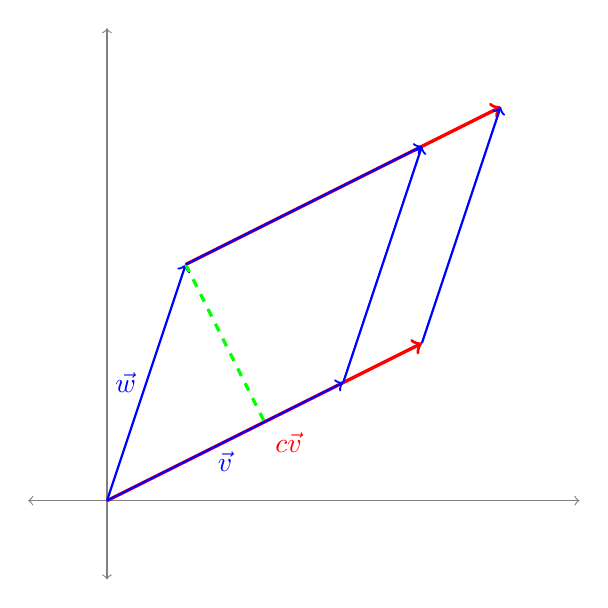
\begin{tikzpicture}
\draw[thin,gray,<->] (-1,0)-- (6,0);
\draw[thin,gray,<->] (0,-1)-- (0,6);
\draw[very thick,red,->] (0,0) -- node[below right] {$c\vec{v}$}  (4,2);
\draw[very thick,red,->] (1,3) -- (5,5);
\draw[thick,blue,->] (0,0) -- node[below] {$\vec{v}$} (3,1.5);
\draw[thick,blue,->] (0,0) -- node[left] {$\vec{w}$} (1,3);
\draw[green,very thick,dashed] (1,3) -- (2,1);
\draw[thick,blue,->] (3,1.5) -- (4,4.5);
\draw[thick,blue,->] (1,3) -- (4,4.5);


\draw[thick,blue,->] (4,2) -- (5,5);
\end{tikzpicture}
\end{center}

\begin{center}
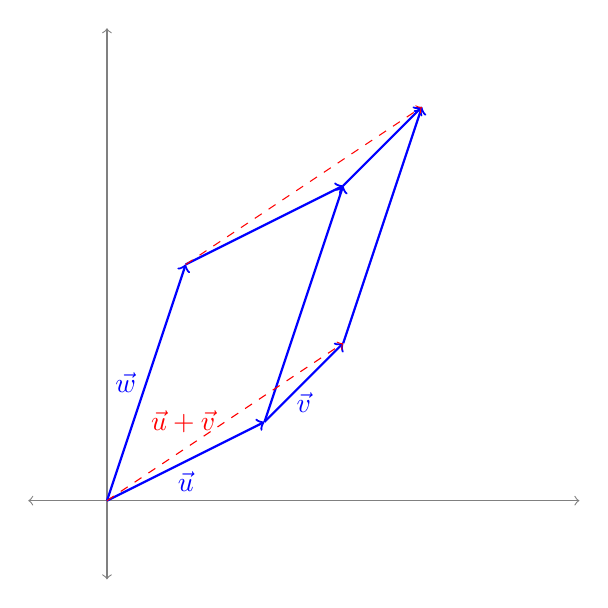
\begin{tikzpicture}
\draw[thin,gray,<->] (-1,0)-- (6,0);
\draw[thin,gray,<->] (0,-1)-- (0,6);
\draw[thick,blue,->] (0,0) -- node[below] {$\vec{u}$} (2,1);
\draw[thick,blue,->] (0,0) -- node[left] {$\vec{w}$} (1,3);
\draw[thick,blue,->] (2,1) -- node [below] {$\vec{v}$}(3,2);
\draw[thick,blue,->] (2,1) -- (3,4);
\draw[thick,blue,->] (3,2) -- (4,5);
\draw[thick,blue,->] (1,3) -- (3,4);
\draw[thick,blue,->] (3,4) -- (4,5);
\draw[dashed,red,->] (0,0) -- node[above,left] {$\vec{u}+\vec{v}$} (3,2);
\draw[dashed,red,->] (1,3) -- (4,5);
\end{tikzpicture}
\end{center}

\end{multicols}
\end{minipage}

\end{activity}

\begin{activity}{10}
What can you conclude about each of the following?
\begin{enumerate}
\item $\det(\vec{e}_1,\vec{e}_2)$
\item $\det(\vec{v},\vec{v})$
\item $\det(c\vec{v},\vec{w})$
\item $\det(\vec{u}+\vec{v},\vec{w})$
\end{enumerate}
\end{activity}


\begin{definition}
To summarize, we have 3 properties (stated here over $\IR^n$)
\begin{enumerate}
\item [P1:] $\det(\vec{e}_1,\vec{e}_2,\ldots,\vec{e}_n)=1$
\item [P2:] If $\vec{v}_i = \vec{v}_j$ for some $i \neq j$, then $\det(\vec{v}_1,\vec{v}_2,\ldots,\vec{v}_n)=0$.
\item[P3:] The determinant is linear in each column.
\end{enumerate}

These three properties uniquely define the \term{determinant}, as we shall see.
\end{definition}

\begin{observation}
Note that if $\vec{v},\vec{w} \in \IR^2$ and $A=\begin{bmatrix} \vec{v} & \vec{w}\end{bmatrix}$ we will write either $\det(A)$ or $\det(\vec{v},\vec{w})$ as is convenient.
\end{observation}

\begin{activity}{5}
How are $\det (\vec{v},\vec{w})$ and $\det(\vec{w},\vec{v})$ related?
\begin{enumerate}[(a)]
\item $\det(\vec{v},\vec{w}) = \det(\vec{w},\vec{v})$
\item $\det(\vec{v},\vec{w}) = -\det(\vec{w},\vec{v})$
\item They are unrelated
\item They are related, but not by either (a) or (b).
\end{enumerate}
\end{activity}


\begin{observation}
Note that this implies that the determinant is actually a \textit{signed} area (volume)!
\end{observation}

\begin{activity}{5}
How are $\det (\vec{v}+\vec{w},\vec{w})$ and $\det(\vec{v},\vec{w})$ related?
\begin{enumerate}[(a)]
\item $\det(\vec{v}+\vec{w},\vec{w}) = \det(\vec{v},\vec{w})$
\item $\det(\vec{v}+\vec{w},\vec{w}) = -\det(\vec{v},\vec{w})$
\item They are unrelated
\item They are related, but not by either (a) or (b).
\end{enumerate}
\end{activity}

\begin{observation}
  Note that we now understand the effect of any column operation on the determinant.
\end{observation}


\end{applicationActivities}
